\section{Příklad 2}
% Jako parametr zadejte skupinu (A-H)
\druhyZadani{C}

%%% Krok 1 
\begin{center}
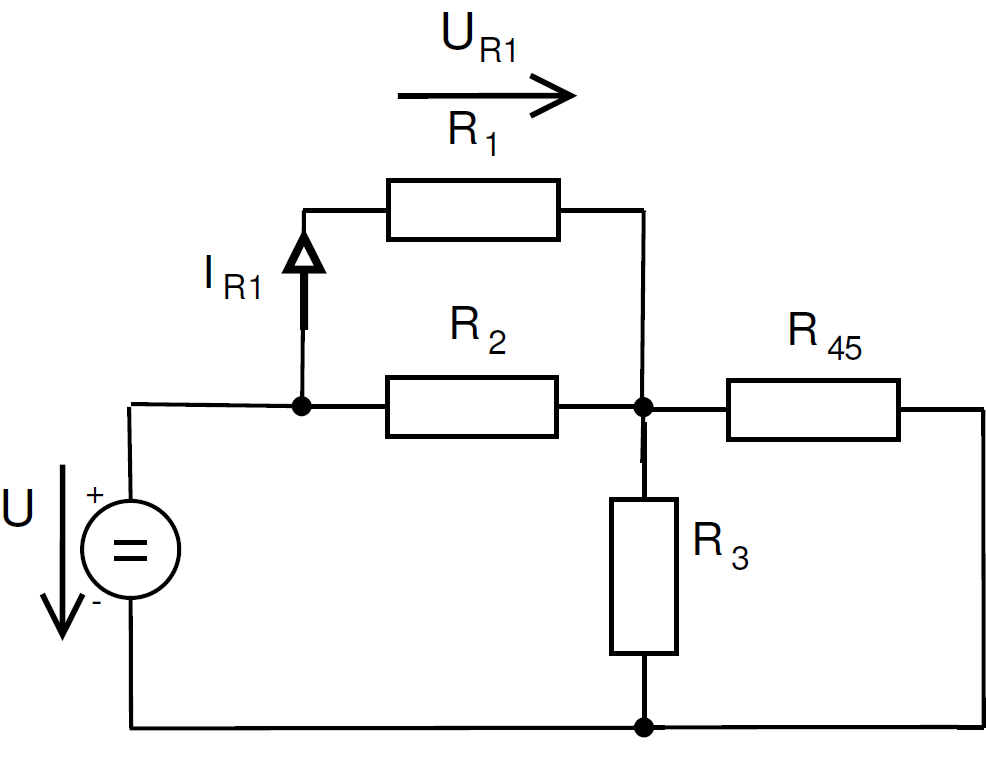
\includegraphics[scale=0.5,keepaspectratio]{fig/obr/Pr2_1.png} \\
\textbf{Krok 1} - Zjednodušenie $R_{4}$ a $R_{5}$ podľa vzorca pre sériovo zapojené rezistory.
\end{center}

\begin{gather*}
R_{45}=R_{4} + R_{5}=690\Omega 
\end{gather*}


%%% Krok 2
\begin{center}
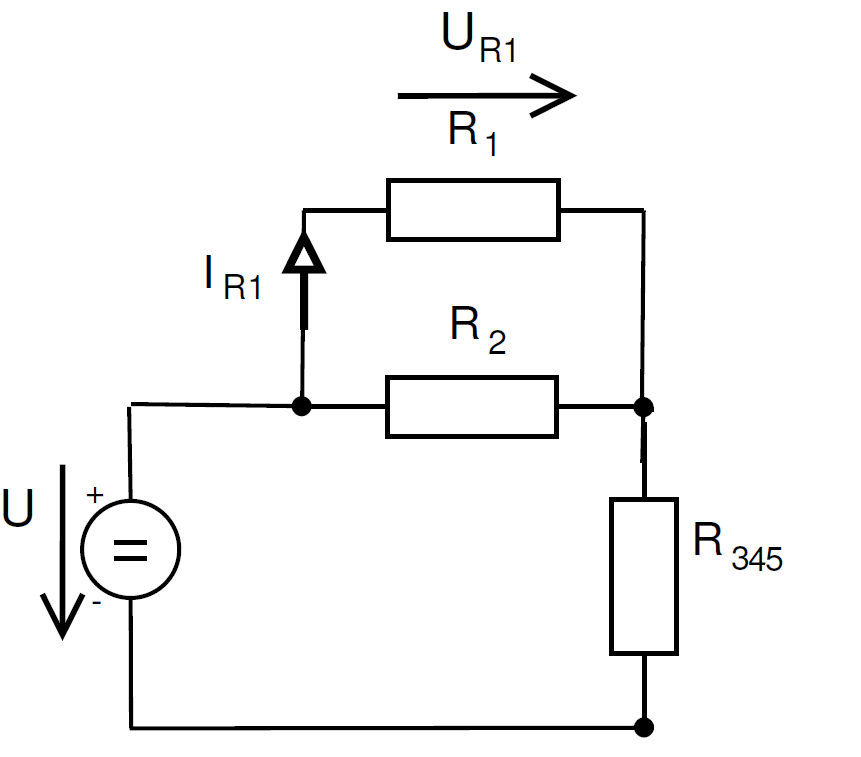
\includegraphics[scale=0.5,keepaspectratio]{fig/obr/Pr2_2.png} \\
\textbf{Krok 2} - Zjednodušenie $R_{45}$ a $R_{3}$ podľa vzorca pre paralelne zapojené rezistory.
\end{center}

\begin{gather*}
R_{345}=\frac{R_{45} \times R_{3}}{R_{45}+R_{3}}=329,3182\Omega 
\end{gather*}


%%% Krok 3
\begin{center}
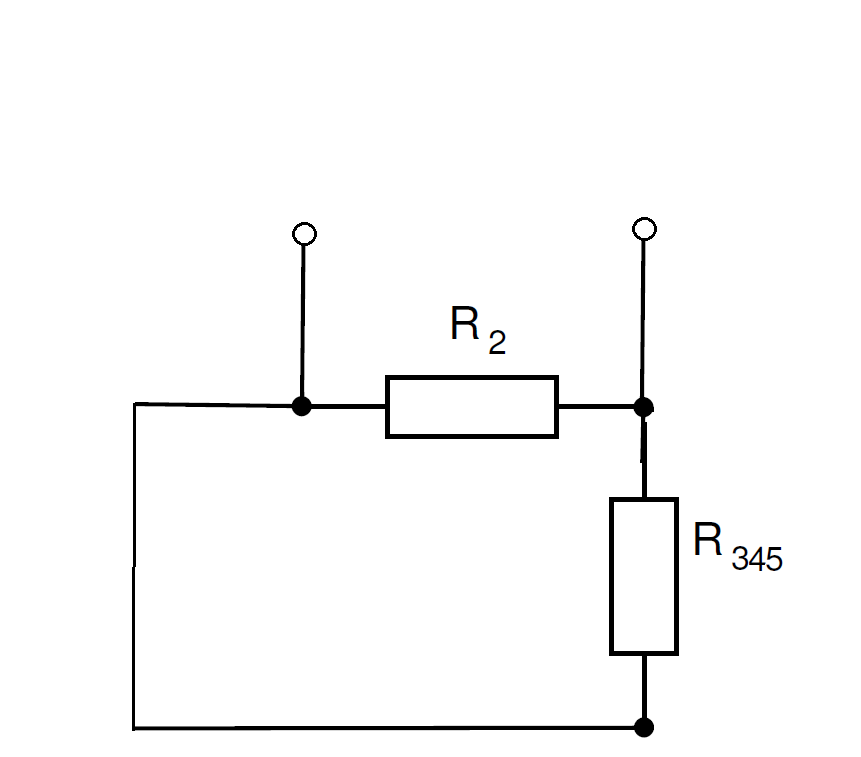
\includegraphics[scale=0.5,keepaspectratio]{fig/obr/Pr2_3.png} \\
\textbf{Krok 3} - Skratovanie zdroja a spočítanie vnútorného odporu $R_{i}$ bez odporu $R_{1}$. Zjednodušenie $R_{2}$ a $R_{345}$.
\end{center}

\begin{gather*}
R_{i}=\frac{R_{2} \times R_{345}}{R_{2}+R_{345}}=\frac{220 \times 329,3182}{220+329,3182}=131,8908\Omega 
\end{gather*}

\newpage

%%% Krok 4
\begin{center}
\textbf{Krok 4} - Vypočítame $U_{i}$.
\end{center}

\begin{gather*}
U_{i}=U \times \frac{R_{2}}{R_{2}+R_{345}}=200 \times \frac{220}{220+329,3182}=80,0993V 
\end{gather*}

%%% Krok 5
\begin{center}
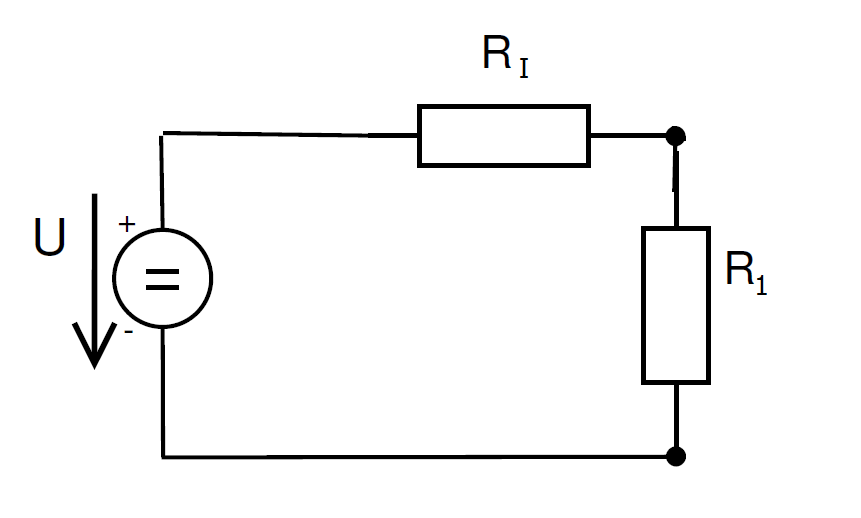
\includegraphics[scale=0.5,keepaspectratio]{fig/obr/Pr2_4.png} \\
\textbf{Krok 5} - Dopočítame  $\boldsymbol{I_{R1}}$ a  $\boldsymbol{U_{R1}}$:
\end{center}

\begin{gather*}
I_{R_{1}}=\frac{U_{i}}{R_{i}+R_{1}}=\frac{80,0993}{131,8908+70}=0,3967A \\
U_{R_{1}}=I_{R_{1}} \times R_{1}=0,3967*70=27,7690V\\
\end{gather*}
